\documentclass[11pt]{article}

% basic packages
\usepackage[margin=1in]{geometry}
\usepackage[pdftex]{graphicx}
\usepackage{amsmath,amssymb,amsthm}
\usepackage{custom}
\usepackage{lipsum}

\usepackage{xcolor}
\usepackage{tikz}

\usepackage[most]{tcolorbox}

% page formatting
\usepackage{fancyhdr}
\pagestyle{fancy}

\renewcommand{\sectionmark}[1]{\markright{\textsf{\arabic{section}. #1}}}
\renewcommand{\subsectionmark}[1]{}
\lhead{\textbf{\thepage} \ \ \nouppercase{\rightmark}}
\chead{}
\rhead{}
\lfoot{}
\cfoot{}
\rfoot{}
\setlength{\headheight}{14pt}

\linespread{1.03} % give a little extra room
\setlength{\parindent}{0.2in} % reduce paragraph indent a bit
\setcounter{secnumdepth}{2} % no numbered subsubsections
\setcounter{tocdepth}{2} % no subsubsections in ToC


%%%%%%%%%%%%%%%%%%%%%%%%%%%%%%%%%%%%%%%%%%%%%%%%%%%%%%%%%%%%%%%%%
% CUSTOM BOXES AND STUFF
\newtcolorbox{redbox}{colback=red!5!white,colframe=red!75!black}
\newtcolorbox{bluebox}{colback=blue!5!white,colframe=blue!75!black}
%%%%%%%%%%%%%%%%%%%%%%%%%%%%%%%%%%%%%%%%%%%%%%%%%%%%%%%%%%%%%%%%%


\begin{document}

% make title page
\thispagestyle{empty}
\bigskip \
\vspace{0.1cm}

\begin{center}
{\fontsize{22}{22} \selectfont Physics Directed Reading Program}
\vskip 16pt
{\fontsize{36}{36} \selectfont \bf \sffamily Topology and Geometry in Physics}
\vskip 24pt
{\fontsize{18}{18} \selectfont \rmfamily Keshav Balwant Deoskar} 
\vskip 6pt
{\fontsize{14}{14} \selectfont \ttfamily kdeoskar@berkeley.edu} 
\vskip 24pt
\end{center}

% {\parindent0pt \baselineskip=15.5pt \lipsum[1-4]} 

% make table of contents
% \newpage

These are some notes from the Phyiscs Directed Reading Program (PDRP) group headed by graduate student Vi Hong. Our group was interested in learning about topology and geometry with applications (primarily) to condensed matter physics.   

\vskip 0.5cm
I'm writing these notes primarily to flesh out my own understanding, and so there's some content I've added which may not have actually been covered in the reading group. The order of topics may also be slightly different.

\vskip 0.5cm
\begin{redbox}
    Please feel free to point out and errors / suggestions if you spot any via email! There's likely to be at least a few. 
\end{redbox}

% \microtoc
\tableofcontents 

% main 

%%%%%%%%%%%%%%%%%%%%%%%%%%%%%%%%%%%%%%%%%%%%%%
\newpage
\section{Review of Topology}
%%%%%%%%%%%%%%%%%%%%%%%%%%%%%%%%%%%%%%%%%%%%%%
\vskip 0.5cm


%%%%%%%%%%%%%%%%%%%%%%%%%%%%%%%%%%%%%%%%%%%%%%
\newpage
\section{Path Integrals and Functional Quantization}
%%%%%%%%%%%%%%%%%%%%%%%%%%%%%%%%%%%%%%%%%%%%%%

\vskip 0.5cm
\subsection{Quick Recap of Lagrangians and Hamiltonians}

The Newtonian Formulation of classical mechanics is amazing but sometimes inconvenient to use because to study the time-evolution of a system, one needs to solve $\mathbf{F} = m\mathbf{a}$ at each time-step. Two equivalent but more convenient formulations are the \textbf{Lagrangian} and \textbf{Hamiltonian} formulations.

\vskip 0.5cm
Both of these rely on the \textbf{Principle of Stationary Action}, which is the idea that each classical system has a quantity associated with it called its action $S$ and, of all the possible ways the system can evole, the path ($x_{cl}(t)$) it actually follows is the one in which the action is extremized i.e. for small devitations $\delta x_i$ from $x_{cl}(t)$, the resulting change in the action is $\delta S = 0$.

\vskip 0.5cm
We define the \textbf{Lagrangian} of the system to be the function $L(q_k, \dot{q}_k, t)$ such that 
\[ S = \int_{r_i}^{r_f} L(q, \dot{q}_k, t) \]
where $q_k$ represents the (generalized) coordinates of the system.

% [Write more in this section later; for now redirect readers to \href{https://github.com/kdeoskar/notes/blob/main/Physics%20105/Notes.pdf}{Physics 105 Notes}.]

\vskip 0.5cm
As you likely know, in settings with no non-conservative forces, the Lagrangian of a system has the form 
\[ L = K - V \]
where $K, V$ are the Kinetic and Potential energies of the system. [If you're not familiar with this, see \href{https://github.com/kdeoskar/notes/blob/main/Physics%20105/Notes.pdf}{these notes on Analytical Mechanics.} ]


\vskip 0.5cm
The principle of least action is essentially saying that for small variations $\delta x(t)$, the classical path is the one corresponding to 

\[ \frac{\partial}{\partial x(t)} \left[ K(x) - V(x) \right] \]

Lagrangians and the Action will be central to the Path Integral formulation, so let's discuss what exactly this sort of derivative means.

\vskip 0.5cm
\subsection{Functional Derivatives}

We're used to functions like $f(x)$ that take in a number and spit out a number, or even functions like $f(\mathbf{x})$ which take in a vector and output some sort of scalar, vector, or other object type. Now, let's consider functionals, like $F[f]$, which take in functions as inputs and spit out some sort of quantity (usually just a scalar).

\vskip 0.5cm
For instance if we have two points $a, b$ in $\mathbb{R}^2$ and we consider the set of paths $\gamma \text{ : } [0, 1] \rightarrow \mathbb{R}^2$ with $\gamma(0) = a, \gamma(1) = b$, then a functional we're all familiar with is 
\begin{align*}
    F[\gamma] = \int_{0}^{1} \sqrt{\left(\frac{\partial \gamma_x}{\partial t}\right)^2 + \left(\frac{\partial \gamma_y}{\partial t}\right)^2  } dt
\end{align*}

This functional takes in a path and spits out the path's length! And if we tweak the path a litle bit $\gamma(t) \rightarrow \gamma'(t) = \gamma(t) + \delta \gamma(t)$ there is a corresponding change in its length, given by 
\[ \frac{\delta F[\gamma]}{\delta \gamma(t)} \]

\vskip 0.5cm
This sort of fractional derivative is important. In the Lagrangian formulation, we want to find the path $x(t)$ through parameter space which minimizes the action $K[x] - V[x]$. i.e. in order to find the classical path, we want to solve the differential equation

\[  \frac{\delta \left(K[x] - V[x]\right)}{\delta x(t)} = 0 \]

\subsection*{Calculating Functional Derivatives}
For a normal function, the derivative is defined as 

\[v \frac{df}{dx} = \lim_{h \rightarrow 0} \frac{f(x + h) - f(x)}{h} \]

Similarly, for a functional, the \emph{functional derivative} is defined as 

\[ \frac{\delta F}{\delta f(x)} = \lim_{h \rightarrow 0} \frac{F[f(x') + h \delta(x - x')] - F[f(x')]}{h} \]

\begin{bluebox}
    \textbf{What does this formula mean?}
    \vskip 0.5cm
    Find good explanation
\end{bluebox}

% \vskip 0.5cm
% \subsection{(A little bit of) Scalar Field Theory}
% A scalar field is a function $\phi : M \rightarrow \mathbb{R}, \mathbb{C}$ from our base-space to (usually) either the real or complex numbers (more generally, it can be to any \textbf{field}). 

\vskip 0.5cm
\subsection{The two main approaches to QFT}
Quantum Field Theory (QFT) is often said to be the merger of quantum mechanics and special relativity, but it can be thought of more generally as the "Calculus of infinitely many degrees of freedom" \cite{232AdiscussionNotes}. 

\vskip 0.5cm
In it we deal with fields over spacetime i.e. smooth functions $\phi \text{ : } M \rightarrow N$ where $M$ is our space-time manifold and $N$ some target space, but which are quantized.

\vskip 0.5cm
There are two main approaches one can take to QFT:

\begin{itemize}
    \item \textbf{"Canonical" or "Second" Quantization:} In Quantum Mechanics, our dynamical variables and observables are promoted operators whose measured valued are quantized. 
    
    % In Second Quantization, our dynamical variables are instead treated as \emph{labels} and for each measurable quantity we have a corresponding \emph{field} which gets quantized.

    In Canonical Quantization, we instead think of Fields as being the fundamental constituents of the universe, and of particles as just being bundles of energy or momenta of the corresponding field \cite{Weinberg97}.
    
    In this formulation, a central object of study is the \emph{exponential of the Interaction Hamiltonian}. The exponential of an operator is defined in terms of an expansion, and so this formulation of QFT lends itself to perturbative situations. 
    
    \item For non-perturbative settings like QCD, the \textbf{Path Integral Formulation} serves us better. It also more easily lets us view the relations between QFT, Statistical Physics, and critical phenomena \cite{Maggiore05}.
\end{itemize}



\vskip 0.5cm
\subsection{Heauristic view of Path Integrals in Quantum Mechanics}

Consider a double slit experiment in which we have source $S$ at some distance from a screen, and plane between them. Suppose the plane has two slits $A_1$ and $A_2$. Then, the probability that an electron emitted by $S$ reaches a specific point $O$ on the screen is given by (the probability it passes through $A_1$ and reaches $O$) + (the probability it passes through $A_2$ and reaches $O$). 

\vskip 0.5cm
If we have 3 slits $A_1, A_2, A_3$ then the same idea holds but with a term for the probability through $A_3$. Similarly, if we have a \textit{second plane} placed after the first with another set of 3 slits, then we need to consider the probability that the electron passes through $A_{1,i}$ followed by $A_{2,j}$ and then hits $O$.

\vskip 0.5cm
\begin{center}
    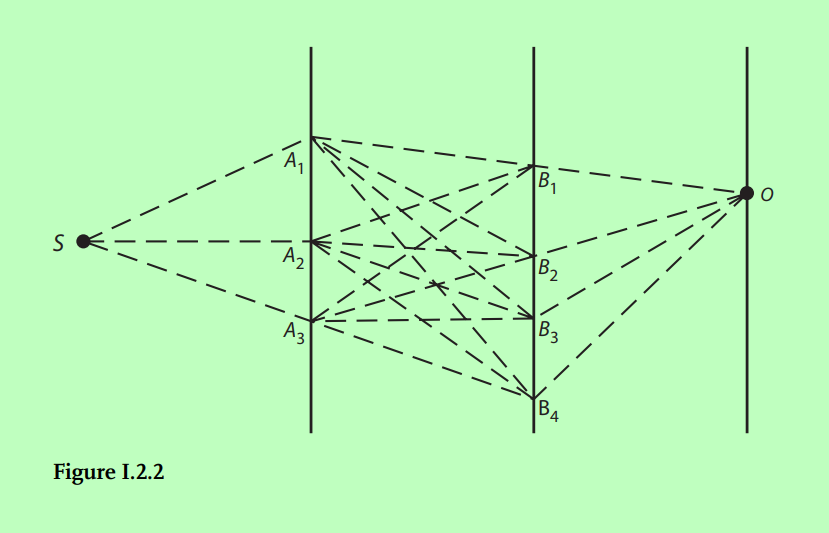
\includegraphics[scale=0.5]{multiple_slits.png} \\
    \textit{Figure 1.2.2 from} \cite[Zee, QFT in a Nutshell]{ZeeQFTNutshell}
\end{center}

\vskip 0.5cm
If we now imagine that the number of holes and the number of planes placed one after another both go to $\infty$ (i.e. we have empty space between $S$ and $O$), then it seems reasonable to say 

\[ \mathcal{A}(S \rightarrow O) =  \sum_{\text{path } \gamma} \mathcal{A}\left(S \rightarrow O \text{ via } \gamma\right) \]

and as we take the limits, this sum over paths made of straight segments approaches an integral over all smooth paths between $S$ and $O$. This is the general idea.


\vskip 0.5cm
\subsection{A... Slightly Less Heauristic View of Path Integrals}



%%%%%%%%%%%%%%%%%%%%%%%%%%%%%%%%%%%%%%%%%%%%%%
\newpage
\section{Fiber Bundles and Principal G-Bundles}
%%%%%%%%%%%%%%%%%%%%%%%%%%%%%%%%%%%%%%%%%%%%%%
\vskip 0.5cm


%%%%%%%%%%%%%%%%%%%%%%%%%%%%%%%%%%%%%%%%%%%%%%
\newpage
\section{Connections on Bundles}
%%%%%%%%%%%%%%%%%%%%%%%%%%%%%%%%%%%%%%%%%%%%%%
\vskip 0.5cm


%%%%%%%%%%%%%%%%%%%%%%%%%%%%%%%%%%%%%%%%%%%%%%
\newpage
\section{Connection 1-forms}
%%%%%%%%%%%%%%%%%%%%%%%%%%%%%%%%%%%%%%%%%%%%%%
\vskip 0.5cm


%%%%%%%%%%%%%%%%%%%%%%%%%%%%%%%%%%%%%%%%%%%%%%
\newpage
\section{TQFTs I}
%%%%%%%%%%%%%%%%%%%%%%%%%%%%%%%%%%%%%%%%%%%%%%
\vskip 0.5cm


%%%%%%%%%%%%%%%%%%%%%%%%%%%%%%%%%%%%%%%%%%%%%%
\newpage
\section{TQFTs II}
%%%%%%%%%%%%%%%%%%%%%%%%%%%%%%%%%%%%%%%%%%%%%%
\vskip 0.5cm


%%%%%%%%%%%%%%%%%%%%%%%%%%%%%%%%%%%%%%%%%%%%%%
\newpage
\section{BRST Quantization}
%%%%%%%%%%%%%%%%%%%%%%%%%%%%%%%%%%%%%%%%%%%%%%
\vskip 0.5cm
Explain stuff.


\vskip 0.5cm
\subsection{BRST Cohomology}

In a theory with gauge-symmetry, we have redundancy. 


%%%%%%%%%%%%%%%%%%%%%%%%%%%%%%%%%%%%%%%%%%%%%%
\newpage
% \section{References}
%%%%%%%%%%%%%%%%%%%%%%%%%%%%%%%%%%%%%%%%%%%%%%
\vskip 0.5cm
\bibliographystyle{plain} % We choose the "plain" reference style
\bibliography{refs} % Entries are in the refs.bib file


\end{document}